\documentclass[12pt,aspectratio=169]{beamer}

% ====================================================
% ====================================================
% USEPACKAGES AND IMPORTS
% ====================================================
% ====================================================

\usepackage[T1]{fontenc}
\usepackage[utf8]{inputenc}
\usepackage[english]{babel}

% tables
\usepackage{tabularx}
\usepackage{colortbl}
\usepackage{multirow}
\usepackage{makecell}

% tikz and colors
\usepackage{tikz}
\usepackage{xcolor}
\usepackage{pgfplots}
\usepackage{pgfplotstable}
\usepackage{tikzsymbols}

\usetikzlibrary{calc}
\usetikzlibrary{trees}
\usetikzlibrary{patterns}
\usetikzlibrary{shadings}
\usetikzlibrary{positioning}
\usetikzlibrary{intersections}
\usepgfplotslibrary{patchplots}
\usepgfplotslibrary{fillbetween}
\usetikzlibrary{decorations.pathreplacing}

\usetikzlibrary{arrows}
\usetikzlibrary{arrows.meta}

\usetikzlibrary{shapes}
\usetikzlibrary{shapes.arrows}
\usetikzlibrary{shapes.callouts}
\usetikzlibrary{shapes.symbols}
\usetikzlibrary{shapes.geometric}

% boxes
\usepackage[many]{tcolorbox}

% math packages and fonts
\usepackage{bm}
\usepackage{ccfonts}
\usepackage{eulervm}
\usepackage{amsmath}
\usepackage{amsfonts}
\usepackage{amssymb}
\usepackage{amsthm}
\usepackage{mathtools}
\usepackage{nicefrac}
\usepackage{slashed}
\usepackage{bbold}
\usepackage{array}
\usepackage{cancel}

% algorithms and listings
\usepackage[ruled,vlined,linesnumbered]{algorithm2e}
\usepackage{listings}
\usepackage{setspace}

\tcbuselibrary{listings}
\tcbuselibrary{breakable}
\tcbuselibrary{skins}

% misc
\usepackage{soul}
\usepackage{pifont}
\usepackage{skull}
\usepackage{multicol}
\usepackage{animate}
\usepackage{hyperref}
\usepackage{wasysym}
\usepackage[absolute,overlay]{textpos}
\usepackage[hang,flushmargin]{footmisc}

% ====================================================
% ====================================================
% LAYOUT AND THEME
% ====================================================
% ====================================================

\usetheme{Copenhagen}

% color definitions
\definecolor{myblue1}{RGB}{35,119,189}
\definecolor{myblue2}{RGB}{95,179,238}
\definecolor{myblue3}{RGB}{129,168,207}
\definecolor{myblue4}{RGB}{26,89,142}

\definecolor{myred1}{RGB}{247,12,12}

% set theme colors
\setbeamercolor*{structure}{fg=myblue1,bg=blue}
\setbeamercolor*{palette primary}{use=structure,fg=white,bg=structure.fg}
\setbeamercolor*{palette secondary}{use=structure,fg=white,bg=structure.fg!75!black}
\setbeamercolor*{palette tertiary}{use=structure,fg=white,bg=structure.fg!50!black}
\setbeamercolor*{palette quaternary}{fg=black,bg=white}

\setbeamertemplate{itemize item}[circle]
\setbeamertemplate{itemize subitem}[circle]
\setbeamertemplate{itemize subsubitem}[circle]

\setbeamertemplate{enumerate item}[circle]
\setbeamertemplate{enumerate subitem}[circle]
\setbeamertemplate{enumerate subsubitem}[circle]

\setbeamercolor{itemize item}{fg=myblue1}
\setbeamercolor{itemize subitem}{fg=myblue1}
\setbeamercolor{itemize subsubitem}{fg=myblue1}

\setbeamertemplate{section in toc}[circle]
\setbeamertemplate{subsection in toc}[circle]
\setbeamerfont{subsection in toc}{size=\scriptsize}

\setbeamercolor{frametitle continuation}{fg=black}

% title graphic -- sap logo and dhbw logo
\titlegraphic{
\includegraphics[scale=0.1]{../03_img/logo_sap}\hspace*{4.75cm}~%
   	
\includegraphics[scale=0.05]{../03_img/logo_dhbw}
}

\makeatletter
% frame title
\defbeamertemplate*{frametitle}{mydefault}[1][left]
{
  	\ifbeamercolorempty[bg]{frametitle}{}{\nointerlineskip}%
  	\nointerlineskip%
 	\@tempdima=\textwidth%
  	\advance\@tempdima by\beamer@leftmargin%
  	\advance\@tempdima by\beamer@rightmargin%
  	\begin{tcolorbox}[
  		enhanced,
  		outer arc=0pt,
  		arc=0pt,
  		boxrule=0pt,
  		top=0pt,
  		bottom=0pt,
  		enlarge left by=-\beamer@leftmargin,
  		enlarge right by=-\beamer@rightmargin,
  		width=\paperwidth,
  		nobeforeafter,
  		interior style={
    			left color=myblue2,
    			right color=white
    		},
  		shadow={0mm}{-0.4mm}{0mm}{black!60,opacity=0.6},    
  		shadow={0mm}{-0.8mm}{0mm}{black!40,opacity=0.4},    
  	]
    	\usebeamerfont{frametitle}%
    	\vbox{}\vskip-1ex%
    	\if@tempswa\else\csname beamer@fte#1\endcsname\fi%
    	\insertframetitle\par%
    	{%
      		\ifx\insertframesubtitle\@empty%
      		\else%
      		{\usebeamerfont{framesubtitle}\usebeamercolor[fg]{black}\insertframesubtitle\strut\par}%
      		\fi
    	}%
    	\vskip-1ex%
    	\if@tempswa\else\vskip-.3cm\fi
  	\end{tcolorbox}%
}

% footline of a frame
\defbeamertemplate*{footline}{mysplit theme}
{%
  	\leavevmode%
  	\hbox{
		\begin{beamercolorbox}[
			wd=.5\paperwidth,ht=2.5ex,dp=1.125ex,leftskip=.3cm plus1fill,rightskip=.3cm
		]{author in head/foot}%
    			\usebeamerfont{author in head/foot}\insertshortauthor\ (\insertinstitute), \insertdate
  		\end{beamercolorbox}%
  		\begin{beamercolorbox}[
			wd=.5\paperwidth,ht=2.5ex,dp=1.125ex,leftskip=.3cm,rightskip=.3cm plus1fil
		]{title in head/foot}%
    			\usebeamerfont{title in head/foot}\insertshorttitle\hfill
    			\insertprefix-\insertframenumber/\inserttotalframenumber\hspace*{0.5em}
  		\end{beamercolorbox}}%
  	\vskip0pt%
}
\makeatother

% ====================================================
% ====================================================
% COMMANDS AND GENERAL DEFINITIONS
% ====================================================
% ====================================================

% page number prefix
\newcommand\insertprefix{}  % empty by default
\newcommand\prefix[1]{\renewcommand\insertprefix{#1}}

% math definitions
% ====================================================
\DeclareMathOperator*{\argmax}{arg\,max}
\DeclareMathOperator*{\argmin}{arg\,min}
\newcommand*\diff{\mathop{}\!\mathrm{d}}

\newcommand*{\vertbar}{\rule[-1ex]{0.5pt}{2.5ex}}
\newcommand*{\horzbar}{\rule[.5ex]{2.5ex}{0.5pt}}

% commands
% ====================================================

% highlight commands
% --------------------------------------------------------------------------------------------------------
% highlight command
\newcommand{\highlight}[1]{\textcolor{myblue1}{\textbf{#1}}}
\newcommand{\highlighttt}[1]{\textcolor{myblue1}{\texttt{#1}}}
\newcommand{\Highlight}[1]{\textcolor{myred1}{\textbf{#1}}}

% blue color boxes (with frame/without frame/without fill)
\newtcolorbox{boxBlue}{colback=myblue1!10!white,colframe=myblue4}
\newtcolorbox{boxBlueNoFrame}{colback=myblue1!10!white,colframe=myblue1!10!white}
\newtcolorbox{boxBlueNoFill}{colback=white,colframe=myblue4}

% font commands
% --------------------------------------------------------------------------------------------------------
\newcommand{\linkstyle}[1]{\underline{\smash{\texttt{#1}}}} 		% style of hyperlinks

% tikz commands
% --------------------------------------------------------------------------------------------------------

% yellow sticky note
\newcommand{\bubble}[3]{
\begin{textblock}{100}(#1, #2)
      	\begin{tikzpicture}
		\node[rectangle,draw=yellow,very thick,fill=yellow!60,align=center] at (0,0) {#3};
	\end{tikzpicture}
\end{textblock}
}

\newcommand{\floattext}[3]{
\begin{textblock}{100}(#1, #2)
      	#3
\end{textblock}
}

\newcommand{\doublecircle}[2]{
	\draw[fill=white,draw=myblue1] (#1,#2) circle (2mm);
	\draw[fill=myblue1,draw=myblue1] (#1,#2) circle (1.5mm);
}

% slide modifiers
% --------------------------------------------------------------------------------------------------------
% mark slide as optional
\newcommand{\optional}{
	\begin{textblock}{100}(0.15,0.30)
      		
\includegraphics[scale=0.2]{../03_img/scream}
    	\end{textblock}
}

% mark slide as important
\newcommand{\important}{
	\begin{textblock}{100}(0.10,0.15)
      		
\includegraphics[scale=0.1]{../03_img/important}
    	\end{textblock}
}

% citation
% --------------------------------------------------------------------------------------------------------
% first argument in {book, online, article}
\newcommand{\literature}[5]{
	\setbeamertemplate{bibliography item}[#1]
	\bibitem{#2}
	\highlight{#3} \\
	\textcolor{darkgray}{\textit{#4}} \\
	\textcolor{black}{#5}
}
% cite content
\newcommand{\citeAuthor}[3]{\vfill\scriptsize\textcolor{lightgray}{#1 \cite{#2} #3}}

% slide architecture
% --------------------------------------------------------------------------------------------------------
% divide frame into two parts
\newcommand{\divideTwo}[4]{
	\begin{minipage}{#1\textwidth}
		#2
	\end{minipage}
	\hfill
	\begin{minipage}{#3\textwidth}
		#4
	\end{minipage}
}

% divide frame into two parts (start on top)
\newcommand{\divideTwoTop}[4]{
	\begin{minipage}[t]{#1\textwidth}
		#2
	\end{minipage}
	\hfill
	\begin{minipage}[t]{#3\textwidth}
		#4
	\end{minipage}
}

% special pages
% --------------------------------------------------------------------------------------------------------
% title page
\newcommand{\maketitlepage}{
	{
		\beamertemplatenavigationsymbolsempty
		\usebackgroundtemplate{%
			\tikz[overlay,remember picture] \node[opacity=0.2, at=(current page.center)] {
  				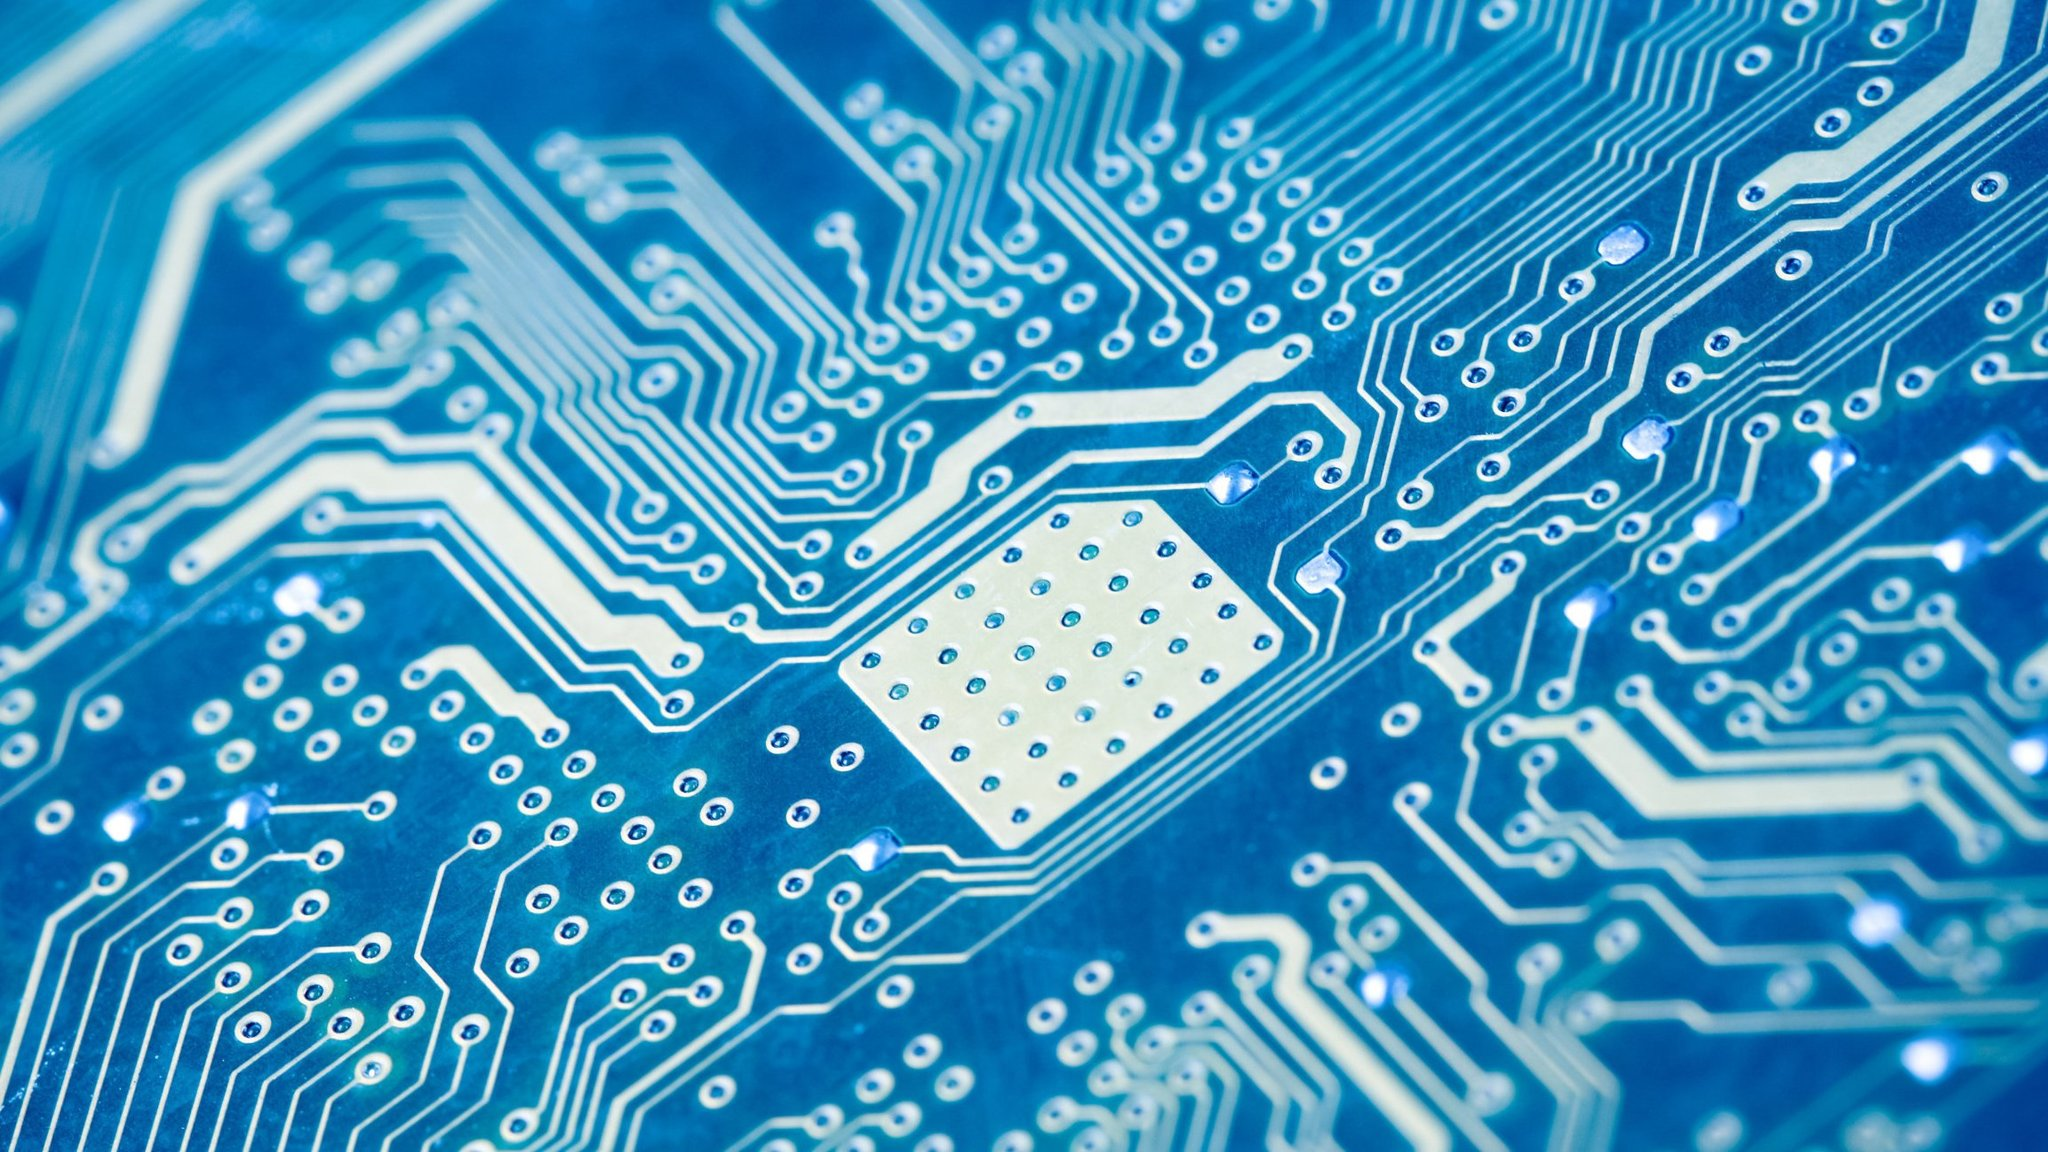
\includegraphics[height=\paperheight,width=\paperwidth]{../03_img/processor.jpg}
			};
		}
		\begin{frame}[plain]
			\vspace*{0.75cm}
			\maketitle
			\vfill
			\begin{center}
				\footnotesize Find all slides on \href{https://github.com/DaWe1992/Applied_ML_Fundamentals}{\linkstyle{GitHub}}
			\end{center}
		\end{frame}
	}
}

% divider page
\newcommand{\makedivider}[1]{
	{
		\beamertemplatenavigationsymbolsempty
		\usebackgroundtemplate{%
			\tikz[overlay,remember picture] \node[opacity=0.2, at=(current page.center)] {
  				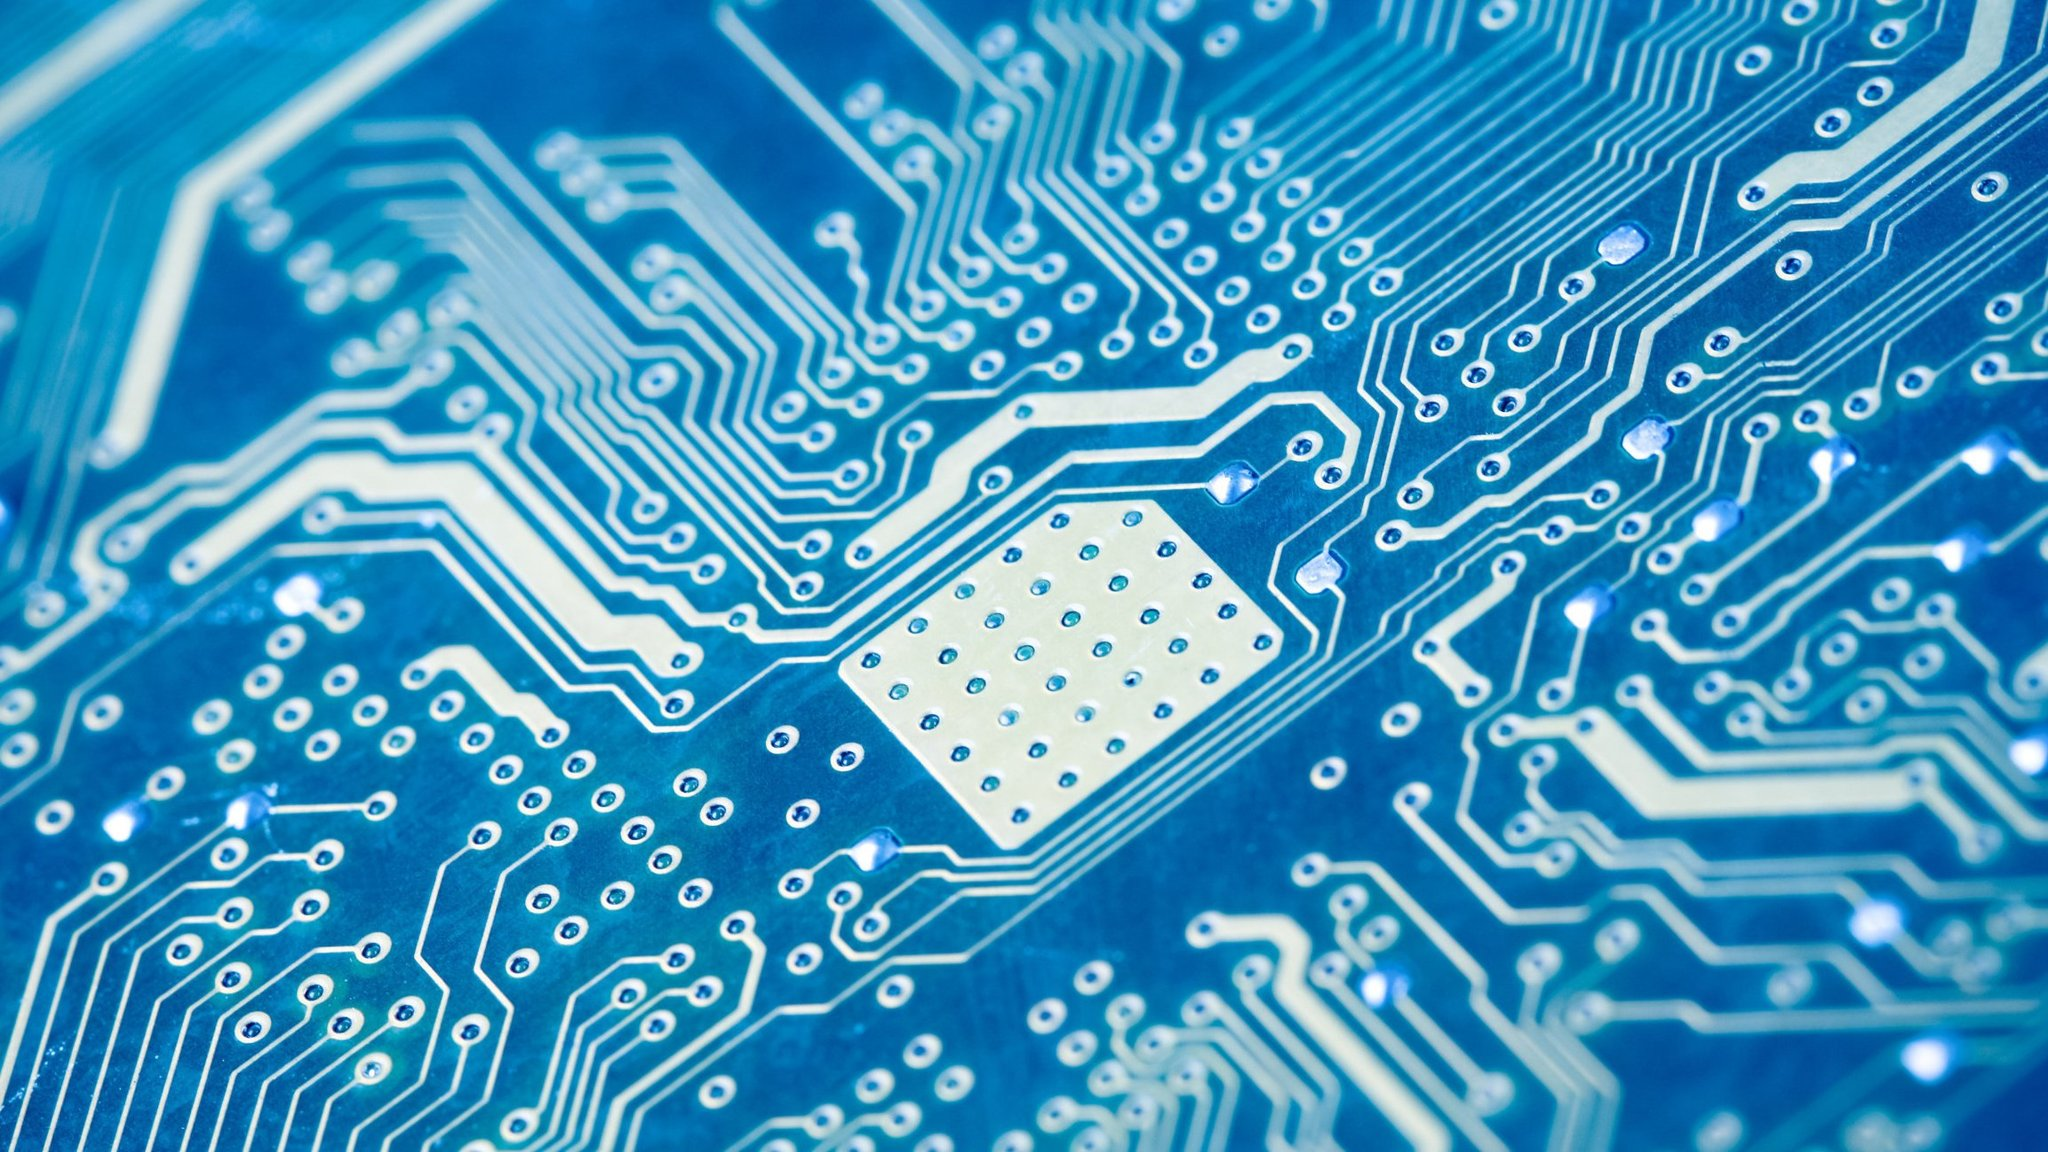
\includegraphics[height=\paperheight,width=\paperwidth]{../03_img/processor.jpg}
			};
		}
		\begin{frame}[plain]
			\vfill
			\begin{boxBlue}
				\centering
				\textbf{Section:} \\
				\large \highlight{#1}
			\end{boxBlue}
			\vfill
			\centering
			
\includegraphics[scale=0.05]{../03_img/logo_dhbw.png}
			\vfill
		\end{frame}
	}
}

% overview page
\newcommand{\makeoverview}[1]{
	\begin{frame}{Lecture Overview}{}
		\begin{tabbing}
			\hspace*{3.5cm}\= \kill
			\ifnum #1=1 \highlight{\textbf{Unit I:}} \else \textbf{Unit I:} \fi
			\> \ifnum #1=1 \highlight{Machine Learning Introduction} \else Machine Learning Introduction \fi \\
		\end{tabbing}
	\end{frame}
}

% thank you page
\newcommand{\makethanks}{
	{\beamertemplatenavigationsymbolsempty
	\begin{frame}[plain]
		\vfill
		\begin{boxBlue}
			\centering
			\Large \highlight{Thank you very much for the attention!}
		\end{boxBlue}
		
		\vfill\footnotesize
		\begin{tabbing}
			\hspace*{1.5cm}\= \kill
			\highlight{Topic:} 	\> \inserttitle \\
			\highlight{Date:} 	\> \insertdate
		\end{tabbing}
		
		\vfill
		\highlight{Contact:} \\
		\insertauthor\ (D062271) \\
		\insertinstitute \\
		\href{mailto:daniel.wehner@sap.com}{\linkstyle{daniel.wehner@sap.com}}
		
		\vfill\normalsize
		\begin{center}
			\large\highlight{Do you have any questions?}
		\end{center}
		\vfill
	\end{frame}}
}

% global pfgplots settings
% --------------------------------------------------------------------------------------------------------
\pgfplotsset{
	% allow filtering of data for pgfplots
	discard if/.style 2 args={
        		x filter/.code={
            		\edef\tempa{\thisrow{#1}}
            		\edef\tempb{#2}
            		\ifx\tempa\tempb
                		\def\pgfmathresult{inf}
            		\fi
        		}
    	},
    	discard if not/.style 2 args={
        		x filter/.code={
            		\edef\tempa{\thisrow{#1}}
            		\edef\tempb{#2}
            		\ifx\tempa\tempb
            		\else
                		\def\pgfmathresult{inf}
            		\fi
        		}
    	}
}


% ====================================================
% ====================================================
% PRESENTATION DATA
% ====================================================
% ====================================================

\title[Deep Learning]{*** Applied Machine Learning Fundamentals *** Neural Networks / Deep Learning}
\institute{SAP\,SE}
\author{M.\,Sc. Daniel Wehner}
\date{Winter term 2019/2020}
\prefix{DL}

% ====================================================
% ====================================================
% BEGIN OF DOCUMENT
% ====================================================
% ====================================================

\begin{document}

% Title frame
%______________________________________________________________________
\maketitlepage


% Lecture Overview
%______________________________________________________________________
\begin{frame}{Lecture Overview}{}
	\makeoverview{8}
\end{frame}


% Agenda
%______________________________________________________________________
\begin{frame}{Agenda for this Unit}
	\begin{multicols}{2}
		\tableofcontents
	\end{multicols}
\end{frame}


% Section: Introduction
%______________________________________________________________________
\section{Introduction}
\makedivider{Introduction}

% Subsection: What is Deep Learning?
% --------------------------------------------------------------------------------------------------------
\subsection{What is Deep Learning?}

% What is Deep Learning?
\begin{frame}{What is Deep Learning?}{}
	\begin{itemize}
		\item `Deep Learning' is a fancy new term for `artificial neural networks' 
		\item It is a \textbf{supervised} method and \textbf{model based}
		\item Artificial neural networks are inspired by the human brain
		\item Lots of different architectures exist:
		\begin{itemize}
			\item \highlight{Multi-Layer perceptrons (MLPs)}
			\item \highlight{Radial Basis Function Networks (RBFNs)}
			\item \highlight{Convolutional neural networks (CNNs, ConvNets)}
			\item \highlight{Recurrent neural networks (LSTMs, GRUs, etc.)}
			\item \highlight{Residual networks (ResNets)}
		\end{itemize}
	\end{itemize}
\end{frame}


% Subsection: History of Deep Learning?
% --------------------------------------------------------------------------------------------------------
\subsection{History of Deep Learning}

% History of Deep Learning
\begin{frame}{History of Deep Learning}{}
	\footnotesize
	\divideTwo{0.49}{
		\begin{boxBlueNoFrame}
			\textbf{Early booming} (1950s -- early 1960s) \\

			\textit{F. Rosenblatt} suggests the \highlight{Perceptron} learning algorithm:
				\href{https://blogs.umass.edu/brain-wars/files/2016/03/rosenblatt-1957.pdf}{\linkstyle{Click here!}}
		\end{boxBlueNoFrame}
	}{0.49}{
		\begin{boxBlueNoFrame}
			\begin{figure}
				\centering
				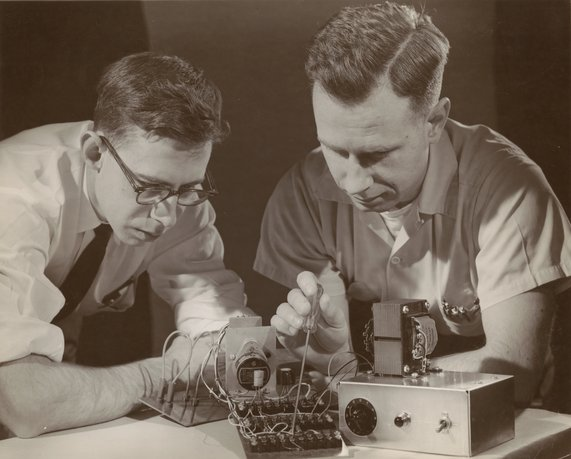
\includegraphics[scale=0.875]{10_deep_learning/02_img/perceptron_rosenblatt}
			\end{figure}
		\end{boxBlueNoFrame}
	}

	\divideTwo{0.49}{
		\begin{boxBlueNoFrame}
			\begin{figure}
				\centering
				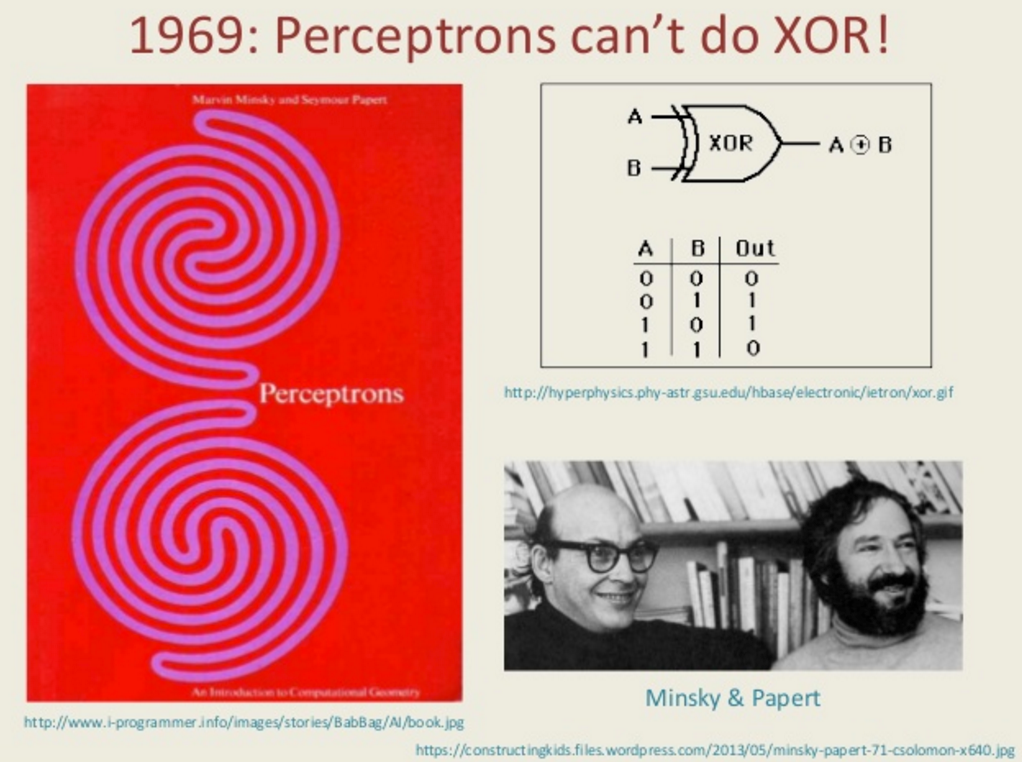
\includegraphics[scale=0.19]{10_deep_learning/02_img/perceptron_xor}
			\end{figure}
		\end{boxBlueNoFrame}
	}{0.49}{
		\begin{boxBlueNoFrame}
			\textbf{Setback I} (mid 1960s -- late 1970s) \\

			\textit{M.\,Minsky} and \textit{S.\,Papert} (1969): \\
			Serious problems with perceptron algorithm.
			It cannot learn the \textbf{XOR problem}.
		\end{boxBlueNoFrame}
	}
\end{frame}


% History of Deep Learning (Ctd.)
\begin{frame}{History of Deep Learning (Ctd.)}{}
	\footnotesize
	\divideTwo{0.49}{
		\begin{boxBlueNoFrame}
			\textbf{Renewed enthusiasm} (1980s)
			\begin{itemize}
				\setlength\itemsep{0.15em}
				\item New techniques available
				\item \highlight{Backpropagation} for deep nets
			\end{itemize}	
		\end{boxBlueNoFrame}

		\begin{boxBlueNoFrame}
			\textbf{Setback II} (1990s -- mid 2000s)
			\begin{itemize}
				\setlength\itemsep{0.15em}
				\item Other techniques were considered superior (e.\,g. SVMs)
				\item CS journals rejected papers on neural networks
			\end{itemize}
		\end{boxBlueNoFrame}
	}{0.49}{
		\begin{boxBlue}
			\textbf{`Deep Learning'} (since mid 2000) \\

			More data, faster computers, better optimization techniques...

			\begin{figure}
				\centering
				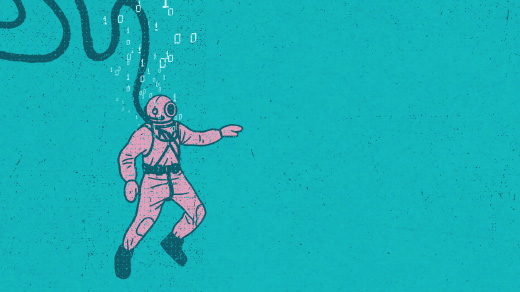
\includegraphics[scale=0.275]{10_deep_learning/02_img/deep_learning}
			\end{figure}
		\end{boxBlue}
	}
\end{frame}


% Subsection: Biological Motivation
% --------------------------------------------------------------------------------------------------------
\subsection{Biological Motivation}

% Biological Motivation
\begin{frame}{Biological Motivation}{}
	\begin{itemize}
		\item All neurons are connected and form a complex \textbf{network}
		\item \textbf{Transmitter chemicals} within the fluid of the brain influence the
			\textbf{electrical potential} inside the body of the neurons
		\item If the \textbf{membrane potential} reaches some threshold the neurons \textbf{fires}
			$\Rightarrow$ A pulse of fixed length is sent down the \textbf{axon}
		\item The axon connects the neuron with other neurons (via \textbf{synapses})
		\item Probably there are 100 trillion \textcolor{red}{\textbf{(!!!)}} synapses in the human brain
		\item \textbf{Refractory period} after a neuron has fired
	\end{itemize}
\end{frame}


% Biological Motivation (Ctd.)
\begin{frame}[plain]{}{}
	\begin{figure}
		\centering
		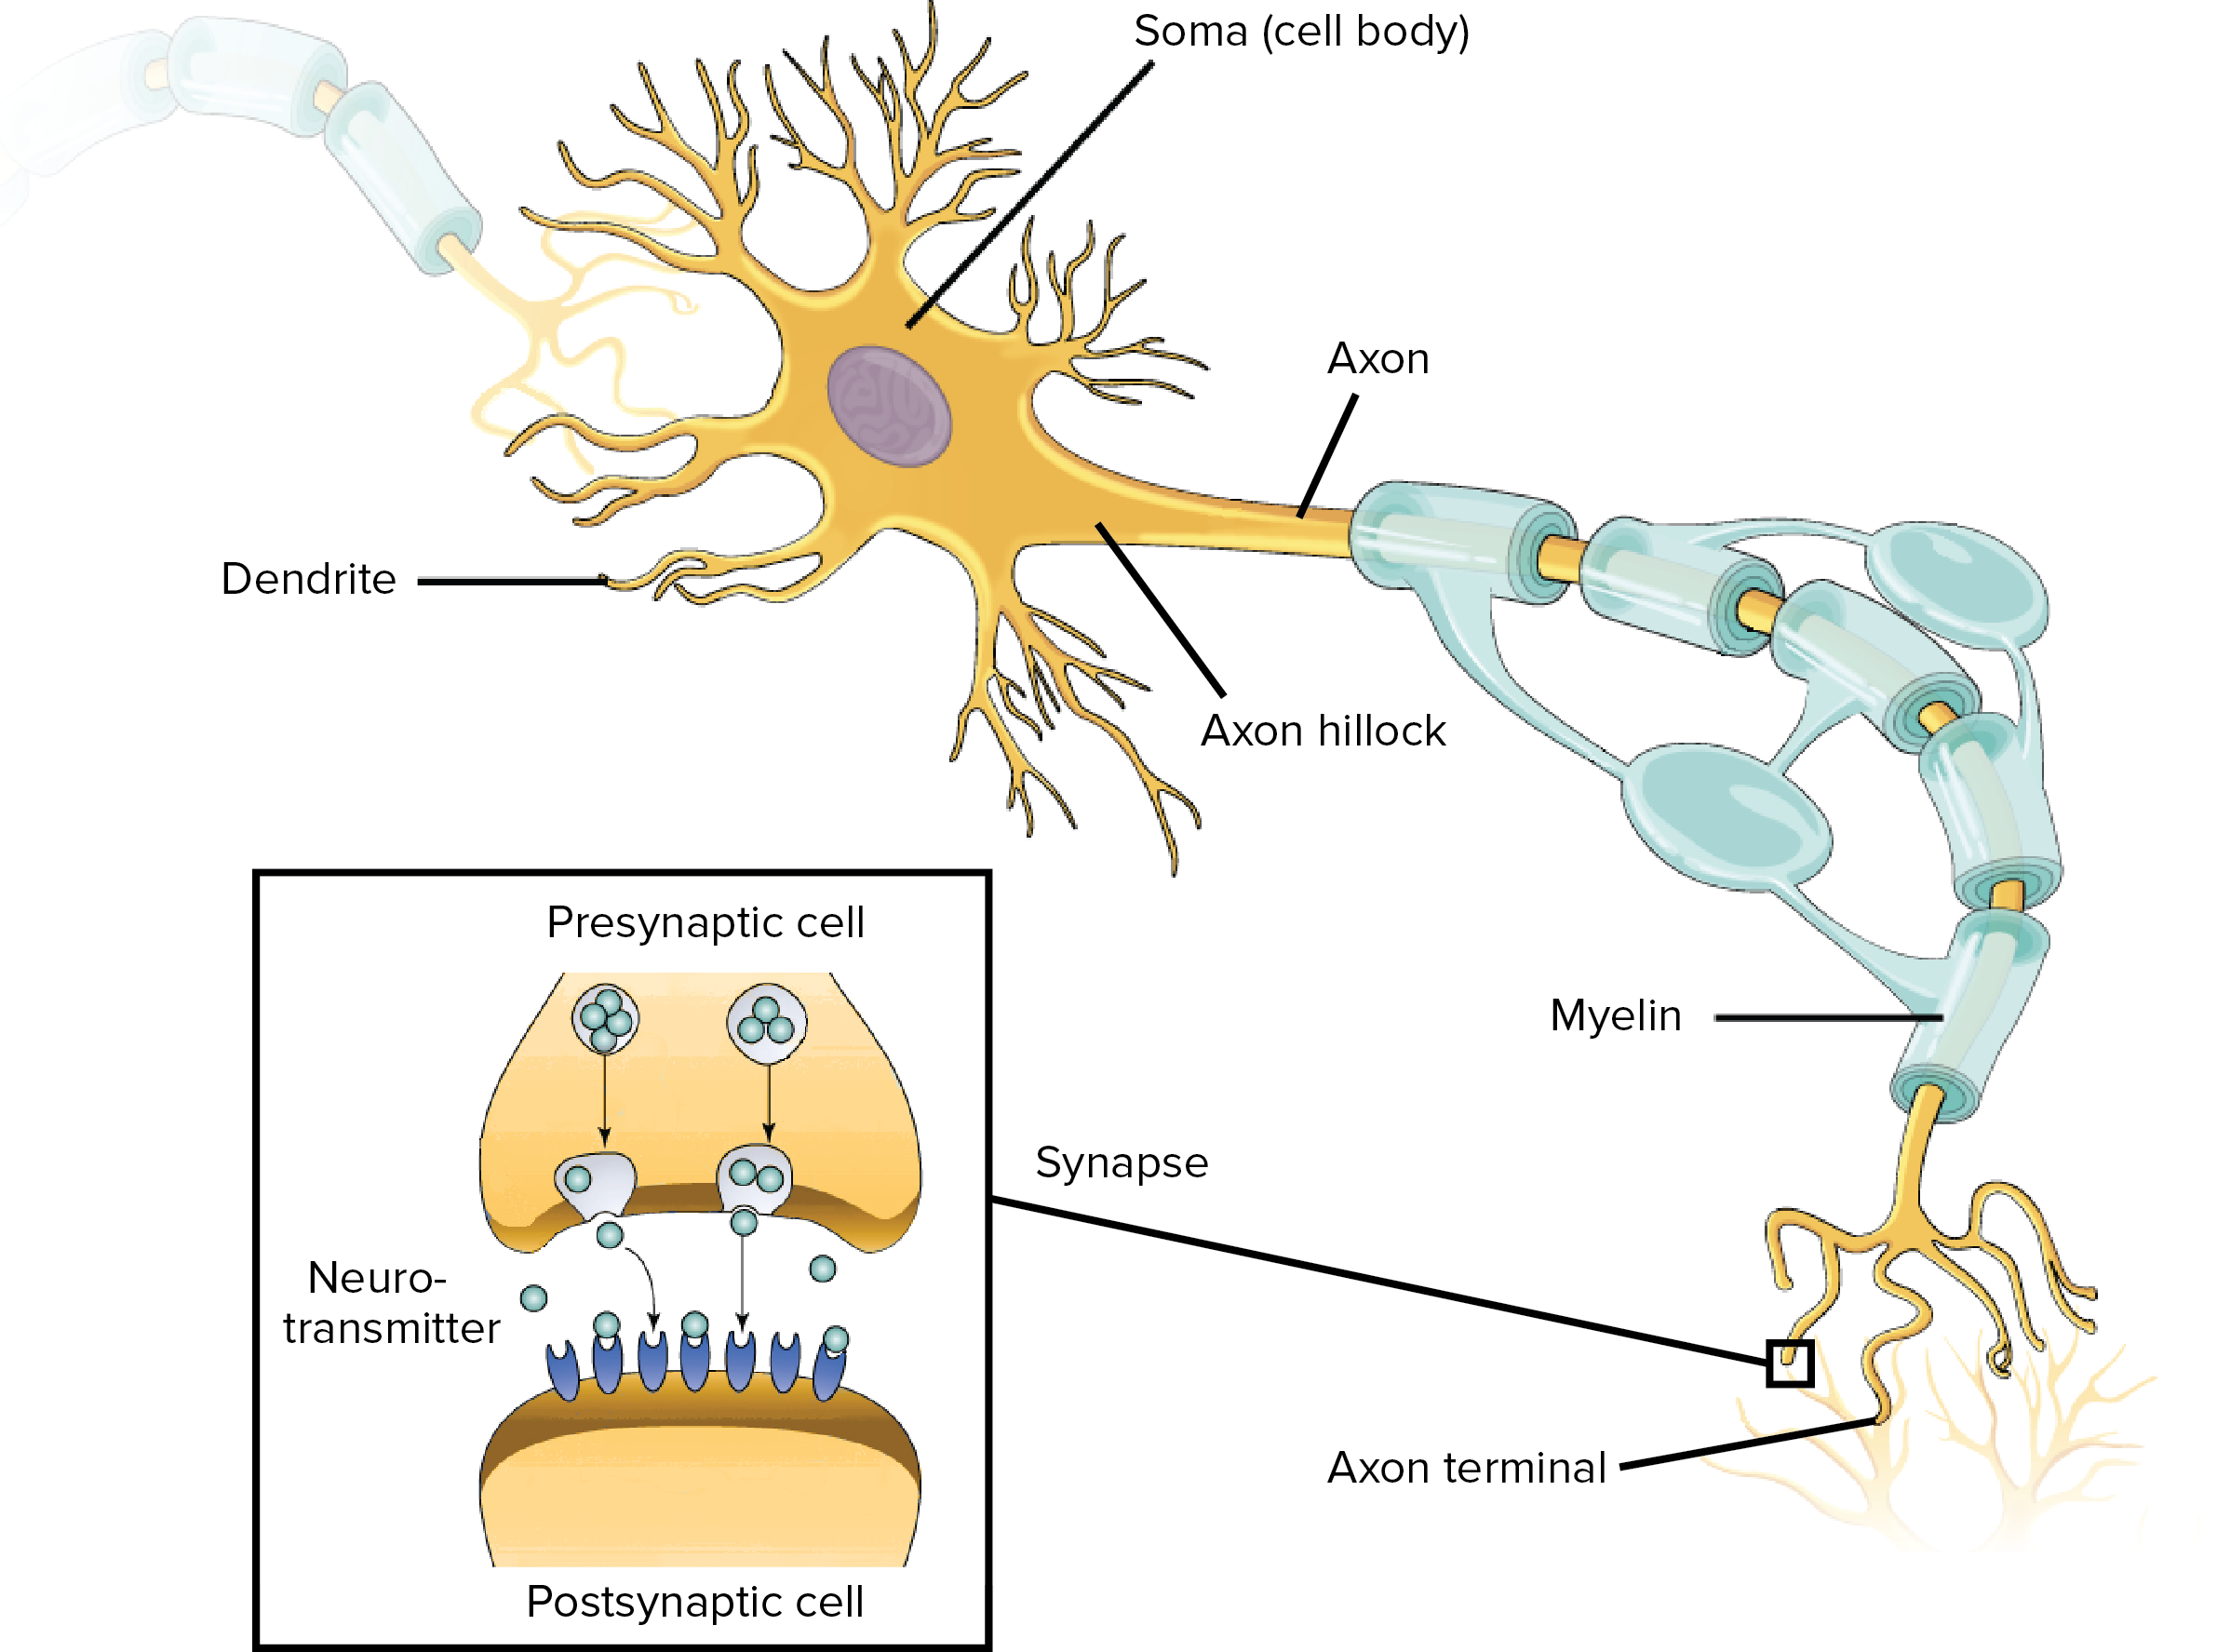
\includegraphics[scale=0.50]{10_deep_learning/02_img/biological_neuron}
	\end{figure}
\end{frame}


% How can we know this?
\begin{frame}{How can we know this?}{}
	\divideTwo{0.39}{
		\begin{figure}
			\centering
			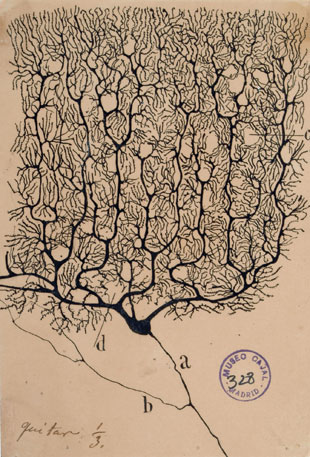
\includegraphics[scale=0.3]{10_deep_learning/02_img/cajal_golgi_stain}
		\end{figure}
	}{0.59}{
		\begin{itemize}
			\item \textit{Santiago Ramón y Cajal} made neurons visible by applying \textbf{Golgi's method}
			\item Golgi's method uses the Golgi stain to colorize the neurons
			\item Cajal establishes the \textbf{neuron doctrine} and won the Nobel price in 1906 for his work
		\end{itemize}
	}
\end{frame}


% How can we know this? (Ctd.)
\begin{frame}{How can we know this? (Ctd.)}{}
	\divideTwo{0.49}{
		\begin{itemize}
			\item End of the 1940s \textit{A. Hodgkin} and \textit{A. Huxley} started investigating the electrical properties of
				neurons on the squid's\footnote[frame]{lat.: \textit{Loligo pealeii}} axon
			\item The right-hand-side image was the first \highlight{action potential} that was plotted
		\end{itemize}
	}{0.49}{
		\begin{figure}
			\centering
			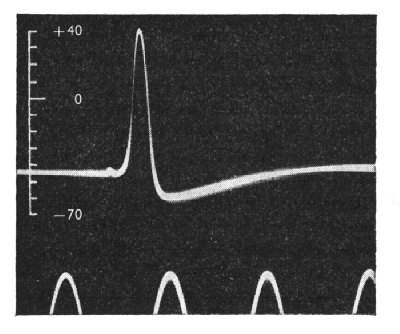
\includegraphics[scale=0.5]{10_deep_learning/02_img/spike_potential_squid}
		\end{figure}
	}
\end{frame}


% How do Humans / Animals learn?
\begin{frame}{How do Humans / Animals learn?}{}
	\footnotesize
	\vspace*{-2mm}
	\begin{itemize}
		\item \textbf{Idea:} Mechanism of learning is \highlight{association}
		\item \highlight{Hebbian learning:} If the firing of one neuron repeatedly assists in firing another neuron
			the synaptic connection will be strengthened
	\end{itemize}
	
	\begin{boxBlueNoFrame}
		\textit{`When an axon of cell A is near enough to excite a cell B and repeatedly or persistently \textbf{takes part in
			firing it}, some growth process or \textbf{metabolic change} takes place in one or both cells such that
			A's \textbf{efficiency}, as one of the cells firing B, is \textbf{increased}.'} \\[-3mm]

		\textit{`The general idea is an old one, that any two cells or systems of cells that are
			\textbf{repeatedly active at the same} time will tend to become \textbf{`associated'}, so that activity
			in one facilitates activity in the other.'} \hfill \textit{Hebb}
	\end{boxBlueNoFrame}
\end{frame}


% Classical / Pavlovian Conditioning
\begin{frame}{Classical / Pavlovian Conditioning}{}
	\footnotesize
	\divideTwo{0.55}{
		\begin{itemize}
			\item Dog salivates when given food
			\item Food is an \highlight{unconditioned stimulus (US)}
			\item Salivation in response to food is \highlight{unconditioned response (UR)}
			\item Food is paired with the sound of a bell
			\item Bell is  \highlight{conditioned stimulus (CS)}
			\item Bell will eventually elicit salivation event without food
			\item Salivation is  \highlight{conditioned response (CR)}
		\end{itemize}
	}{0.43}{
		\begin{figure}
			\centering
			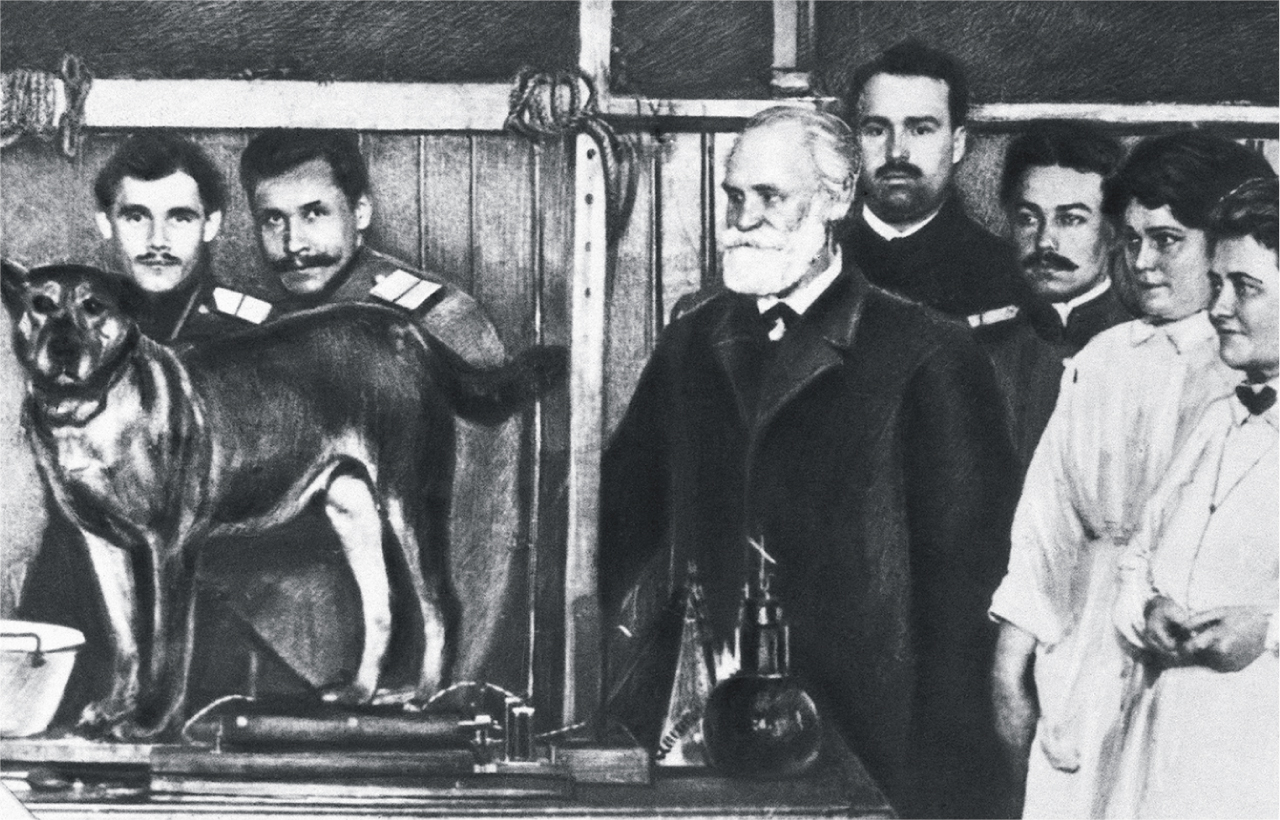
\includegraphics[scale=0.50]{10_deep_learning/02_img/pavlov}
		\end{figure}
	}
\end{frame}


% Classical / Pavlovian Conditioning (Ctd.)
\begin{frame}{Classical / Pavlovian Conditioning (Ctd.)}{}
	\begin{figure}
		\centering
		
\includegraphics[scale=0.70]{10_deep_learning/02_img/pavlov_meme}
	\end{figure}
\end{frame}


% Blocking
\begin{frame}{Blocking}{}
	\begin{table}[h]
	\scalebox{0.75}{
	\begin{tabular}{| l | l | l | l | l |}
		\hline
		\textbf{Group A}	&	train N+	&	train LN+ 	&	test L- 	& 	$\Rightarrow$ no conditioning	\\ \hline
		\textbf{Group B}	&			&	train LN+	&	test L- 	&	$\Rightarrow$ conditioning	\\ \hline
	\end{tabular}}
\end{table}
	
	\footnotesize
	\begin{itemize}
		\item CS is a light (L), a noise (N), or a combination of both (LN)
		\item US is a mild shock that is paired with the CS in the training phase (+)
		\item In all conditions, after training fear response is tested when only L is presented without shock (-)
		\item Group B shows conditioning; Group A does not: \textbf{N blocks L}
		\item This is hard to explain with Hebbian learning
		\item \textbf{Idea:} Learning only happens if there is a \highlight{prediction error}
	\end{itemize}
\end{frame}


% Prediction Error -- Dopamine
\begin{frame}[plain]{}{}
	\begin{figure}
		\centering
		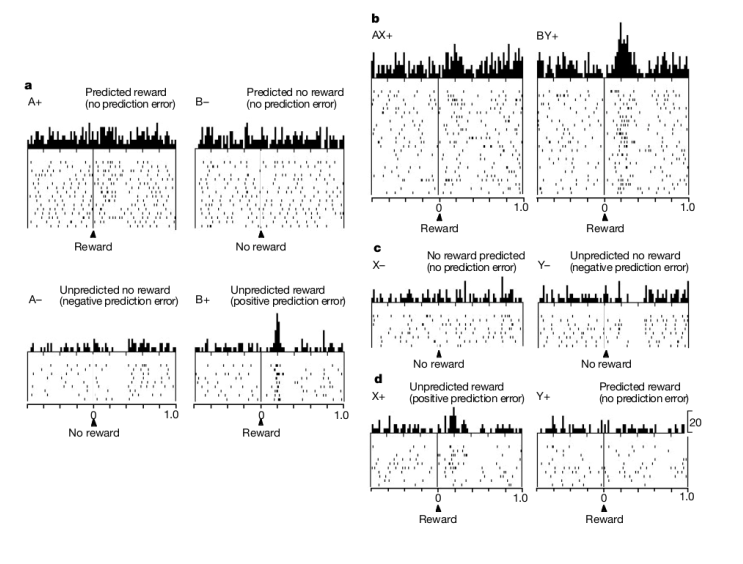
\includegraphics[scale=0.60]{10_deep_learning/02_img/dopamine_prediction_error}
	\end{figure}
\end{frame}


% Artificial Neurons [McCulloch and Pitts 1943]
\begin{frame}{Artificial Neurons [McCulloch and Pitts 1943]}{}
	\begin{itemize}
		\item 1943 \textit{W. S. McCulloch} and \textit{W. H. Pitts} designed the first `artificial neuron'
		\item These neurons can represent logical functions (e.\,g. b -- \texttt{OR}, c -- \texttt{AND})
	\end{itemize}
	
	\begin{figure}
		\centering
		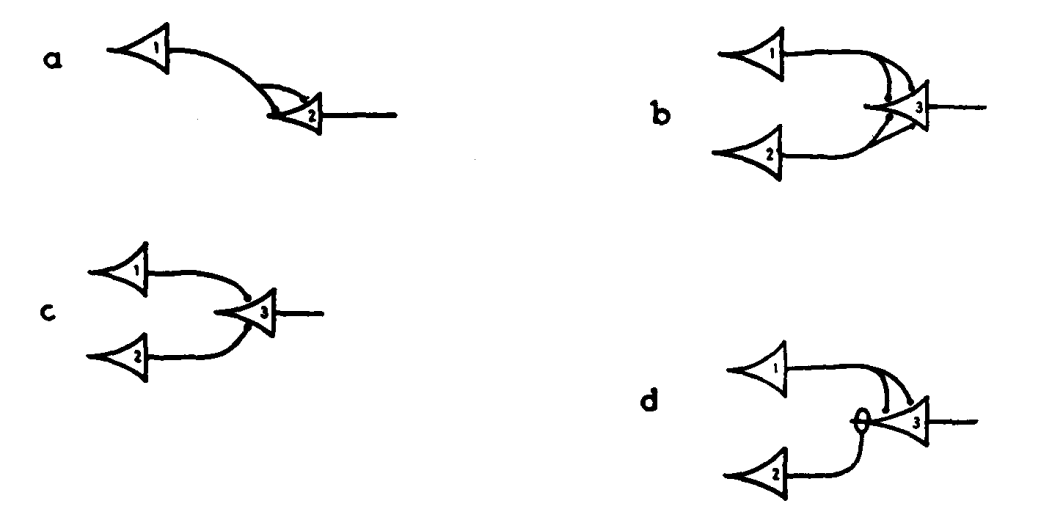
\includegraphics[scale=0.25]{10_deep_learning/02_img/mcculloch_pitts}
	\end{figure}
\end{frame}


% Subsection: Biological Motivation
% --------------------------------------------------------------------------------------------------------
\subsection{Perceptron Learning Algorithm}

% Perceptron [Rosenblatt 1957]
\begin{frame}{Perceptron [Rosenblatt 1957]}{}
	\begin{figure}
	\centering
	\begin{tikzpicture}[
		scale=0.8
	]

		\node[circle,draw=black,minimum size=4cm,thick] (N) at (0,0) {};

		\foreach \y/\i in {1.5/1,0/2,-1.5/3,-3/4}{
			\draw[thick] (-8,\y) -- node[above] {$\theta_{\i}$} (N);
			\node[circle,draw=black,fill=white,thick] at (-8,\y) {$x_{\i}$};
		}

		\draw[thick] (-8,3) -- node[above] {$\theta_{0}$} (N);
		\node[circle,thick,draw=black,fill=black,thick] at (-8,3) {\textcolor{white}{\textbf{1}}};

		\draw[thick] (N) -- ++(6,0) node[right] {z};

		\draw[pattern=north west lines,pattern color=purple!30] (0,2.4) arc (90:270:2.4) -- cycle;
		\draw[pattern=north west lines,pattern color=orange!30] (0,2.4) arc (90:-90:2.4) -- cycle;
		\node at (-1.25,0) {$a = \bm{\theta}^{\intercal} \bm{x}$};
		\node at (1.25,0) {$z = \sigma(a)$};

		\node[purple,align=center] at (-1.15,1) {\scriptsize \textbf{pre-}\\[-2mm] \scriptsize \textbf{activation}};
		\node[orange] at (1.15,1) {\scriptsize \textbf{activation}};
		\node[rotate=90,gray] at (-9,0) {\footnotesize \textbf{input}};
		\node[rotate=90,gray] at (7,0) {\footnotesize \textbf{output}};

	\end{tikzpicture}
\end{figure}
\end{frame}


% Perceptron (Ctd.)
\begin{frame}{Perceptron (Ctd.)}{}
	\begin{itemize}
		\item The neuron receives an input-vector $\bm{x}$
		\begin{equation*}
			\bm{x} = (x_1, x_2, \dots, x_m)^{\intercal}
		\end{equation*}
		\item Each input signal is weighted by a factor\footnote[frame]{weight of synaptic strength} $\theta_j$
		\begin{equation*}
			\bm{\theta} = (\theta_1, \theta_2, \dots, \theta_m)^{\intercal}
		\end{equation*}
		\item We compute the \highlight{pre-activation} and the \highlight{activation}:
		\begin{equation}
			p = \bm{\theta}^{\intercal} \bm{x} + b = \sum_{j=1}^m \theta_j x_j + b \qquad\qquad
			a = \sigma(p)
		\end{equation}
	\end{itemize}
\end{frame}


% Perceptron (Ctd.)
\begin{frame}{Perceptron (Ctd.)}{}
	\begin{itemize}
		\item The simplest activation function is to use a threshold $\rho$:\footnote[frame]{Not used, since not differentiable;
			alternatives later}
		\begin{equation*}
			\sigma(p) =
			\begin{cases}
				0 &	\text{for}\ p \le \rho \\
				1 & \text{for}\ p > \rho
			\end{cases}
		\end{equation*}
		\item Quick example: $\bm{x} = (1, 0, 0.5)^{\intercal}; \bm{\theta} = (1, -0.5, -1)^{\intercal}; \rho = 0$
		\begin{align*}
			p &= \sum_{j=1}^3 \theta_j x_j = 1 \cdot 1 + (-0.5) \cdot 0 + (-1) \cdot 0.5 = 0.5 \\
			a &= \sigma_{\rho=0}(0.5) = 1
		\end{align*}
	\end{itemize}
\end{frame}


% Perceptron Learning
\begin{frame}{Perceptron Learning}{}
	\begin{itemize}
		\item Learning means choosing the correct weights $\bm{\theta}^*$ from a set of possible hypotheses $\mathcal{H}$
		(\highlight{hypothesis space}):
		\begin{equation*}
			\mathcal{H} = \{ \bm{\theta} \vert \bm{\theta} \in \mathbb{R}^m \}
		\end{equation*}
		\item How to learn the weights from a data set $\mathcal{D}$?
		\item \textbf{Algorithm outline:}
		\begin{enumerate}
			\item Pick a training example $\bm{x} \in \mathcal{D}$
			\item Calculate the activation $a$ for that training example
			\item Update the weights $\theta$ based on the error
		\end{enumerate}
	\end{itemize}
\end{frame}


% Perceptron Learning (Ctd.)
\begin{frame}{Perceptron Learning (Ctd.)}{}
	\begin{itemize}
		\item Let the error be denoted by $\delta$
		\item How can we compute the error? We need a loss function $\mathcal{J}(\bm{\theta})$:
		\begin{equation}
			\mathcal{J}(\bm{\theta}) = \frac{1}{2} \sum_{i=1}^N (h_{\bm{\theta}}(\bm{x}^{(i)}) - y^{(i)})^2
		\end{equation}
		\item Again, we use \highlight{gradient descent}: Compute gradient and go into the negative direction:
		\begin{equation}
			\bm{\theta}^{(t+1)} \longleftarrow \bm{\theta}^{(t)} - \alpha \nabla_{\bm{\theta}} \mathcal{J}(\bm{\theta})
		\end{equation}
	\end{itemize}
	\textcolor{gray}{$\Rightarrow$ cf. slides `Regression'}
\end{frame}


% Perceptron Learning Algorithm
\begin{frame}[plain]{}{}
	\begin{algorithm}[H]
		\setstretch{1.1}
		\DontPrintSemicolon
		\footnotesize
		\KwIn{Training data $\mathcal{D}$, convergence threshold $\bm{\varepsilon}$}
		
		\tcp*[h]{initialization}\;
		set all weights $\bm{\theta}^{(0)}$ to small random numbers\;
		\For{$t \in \{0, 1, \dots, \infty\}$}{
			pick a sample $\langle \bm{x}, y \rangle \in \mathcal{D}$ randomly\;
			\tcp*[h]{predict the class label}\;
			compute the activation $a = \sigma(\bm{\theta}^{\intercal} \bm{x})$\;
			\tcp*[h]{stochastic gradient descent: update based on prediction error}\;
			$\bm{\theta}^{(t+1)} \longleftarrow
				\bm{\theta}^{(t)} - \alpha \nabla_{\bm{\theta}} \mathcal{J}(\bm{\theta})$\;
			\If{$\Vert \bm{\theta}^{(t+1)} - \bm{\theta}^{(t)} \Vert \le \bm{\varepsilon}$}{
				\tcp*[h]{convergence}\;
				\textbf{break}\;
			}
		}
		\Return{$\bm{\theta}$}
 		\caption{Perceptron Learning Algorithm}
	\end{algorithm}
\end{frame}


% Perceptron Convergence Theorem
\begin{frame}{Perceptron Convergence Theorem}{}
	\begin{boxBlue}
		\highlight{Perceptron Convergence Theorem} \\

		If the training data is \textbf{linearly separable}, then the perceptron learning algorithm is going to
		\textbf{converge after a finite amount of time} and classifies \textbf{all training data examples correctly}.
	\end{boxBlue}
\end{frame}


% Generalization to multiple Classes
\begin{frame}{Generalization to multiple Classes}{}
	\divideTwo{0.59}{
		\footnotesize
		\begin{itemize}
			\item A single neuron can only distinguish two classes
			\item If there are more than two classes: Simply use more perceptrons\footnote[frame] {This construct is still
				referred to as a perceptron.}
			\item Use \highlight{one-hot encoding} for the classes and \highlight{soft-max} as activation function (later)
			\item Example for three classes:
			\begin{tabbing}
				\hspace*{1cm}\=\kill
				$\mathcal{C}_1$ \> \texttt{1 0 0} \\
				$\mathcal{C}_2$ \> \texttt{0 1 0} \\
				$\mathcal{C}_3$ \> \texttt{0 0 1}
			\end{tabbing}
		\end{itemize}	
	}{0.39}{
		\begin{figure}
	\centering
	\begin{tikzpicture}[
		scale=0.6,
		every node/.style={scale=0.8}
	]

		\foreach \y in {-3,-1.5,0,1.5,3}{
			\foreach \yy in {-2,0,2}{
				\draw (-5,\y) -- (0,\yy);
			}
		}
	
		% input layer
		\foreach \y/\i in {3/1,1.5/2,0/3,-1.5/4,-3/5}{
			\node[circle,draw=black,fill=lightgray] at (-5,\y) {$x_{\i}$};
		}
		
		% rbf layer
		\foreach \y/\i in {-2/3,0/2,2/1}{
			\node[circle,draw=black,fill=white,align=center] at (0,\y) {$P_{\i}$};
		}
		\node at (1.5,2) {\texttt{0}};
		\node at (1.5,0) {\texttt{1}};
		\node at (1.5,-2) {\texttt{0}};

		\node[rotate=90,gray] at (-6.5,0) {\footnotesize \textbf{input}};
		\node[rotate=90,gray] at (2.5,0) {\footnotesize \textbf{output}};

	\end{tikzpicture}
\end{figure}
	}
\end{frame}


% What about non-linear Data Sets?
\begin{frame}{What about non-linear Data Sets?}{}
	\begin{itemize}
		\item If the data is not linearly separable then the perceptron cannot learn it
		\item Remember Marvin Minsky's/Seymour Papert's book \textit{`Perceptrons'}
		\item What can we do?
		\begin{enumerate}
			\item Add feature mapping $\Rightarrow$ \highlight{Radial basis function (RBF) networks}
			\item Add hidden layers $\Rightarrow$ \highlight{Multi-layer perceptrons (MLP)}
		\end{enumerate}
	\end{itemize}
\end{frame}


% Subsection: Radial Basis Function (RBFN) Networks
% --------------------------------------------------------------------------------------------------------
\subsection{Radial Basis Function (RBFN) Networks}

% Radial Basis Function (RBF) Networks
\begin{frame}{Radial Basis Function (RBF) Networks}{}
	\begin{figure}
	\centering
	\begin{tikzpicture}[
		scale=0.8
	]

		\foreach \y in {-3,-1.5,0,1.5,3}{
			\foreach \yy in {-2,0,2}{
				\draw (-5,\y) -- (0,\yy);
			}
		}
	
		% input layer
		\foreach \y/\i in {3/1,1.5/2,0/3,-1.5/4,-3/5}{
			\node[circle,draw=black,fill=lightgray] at (-5,\y) {$x_{\i}$};
		}
		
		% rbf layer
		\foreach \y/\i in {-2/3,0/2,2/1}{
			\draw (0,\y) -- node[above] {$\theta_{\i}$} (5,0);
			\node[circle,draw=black,fill=white,align=center] at (0,\y)
				{\footnotesize $RBF$ \\[-3mm] \tiny $\mu_{\i}, \sigma_{\i}$};
		}

		% output layer
		\draw (5,0) -- ++(2,0);
		\node[circle,draw=black,fill=white] at (5,0) {$P$};
		
	\end{tikzpicture}
\end{figure}
\end{frame}


% Inside an RBF Neuron
\begin{frame}{Inside an RBF Neuron}{}
	\begin{itemize}
		\item Each RBF neuron computes the distance of the input $\bm{x}$ to an \highlight{internal prototype} vector:
		\begin{equation}
			\varphi_j(\bm{x}) = \exp\left\{ -\frac{\Vert \bm{x} - \bm{z_j} \Vert^2}{2\sigma^2} \right\}
		\end{equation}
		\item These distances are then fed into the perceptron
		\item \textbf{How to get the prototypes?}
		\begin{itemize}
			\item We can use clustering, e.\,g. \highlight{k-Means}, to get the locations $\bm{\mu}$ \\
				{\footnotesize (this avoids useless prototypes in areas without data points)}
			\item Choose $\sigma$ neither too small nor too big
		\end{itemize}
		\item There are no weights $\bm{\theta}$ to tune for that neuron
	\end{itemize}
\end{frame}


% Example: Radial Basis Function (RBF) Networks
\begin{frame}[plain]{}{}
	\vspace*{-7mm}
	\begin{figure}
		\centering
		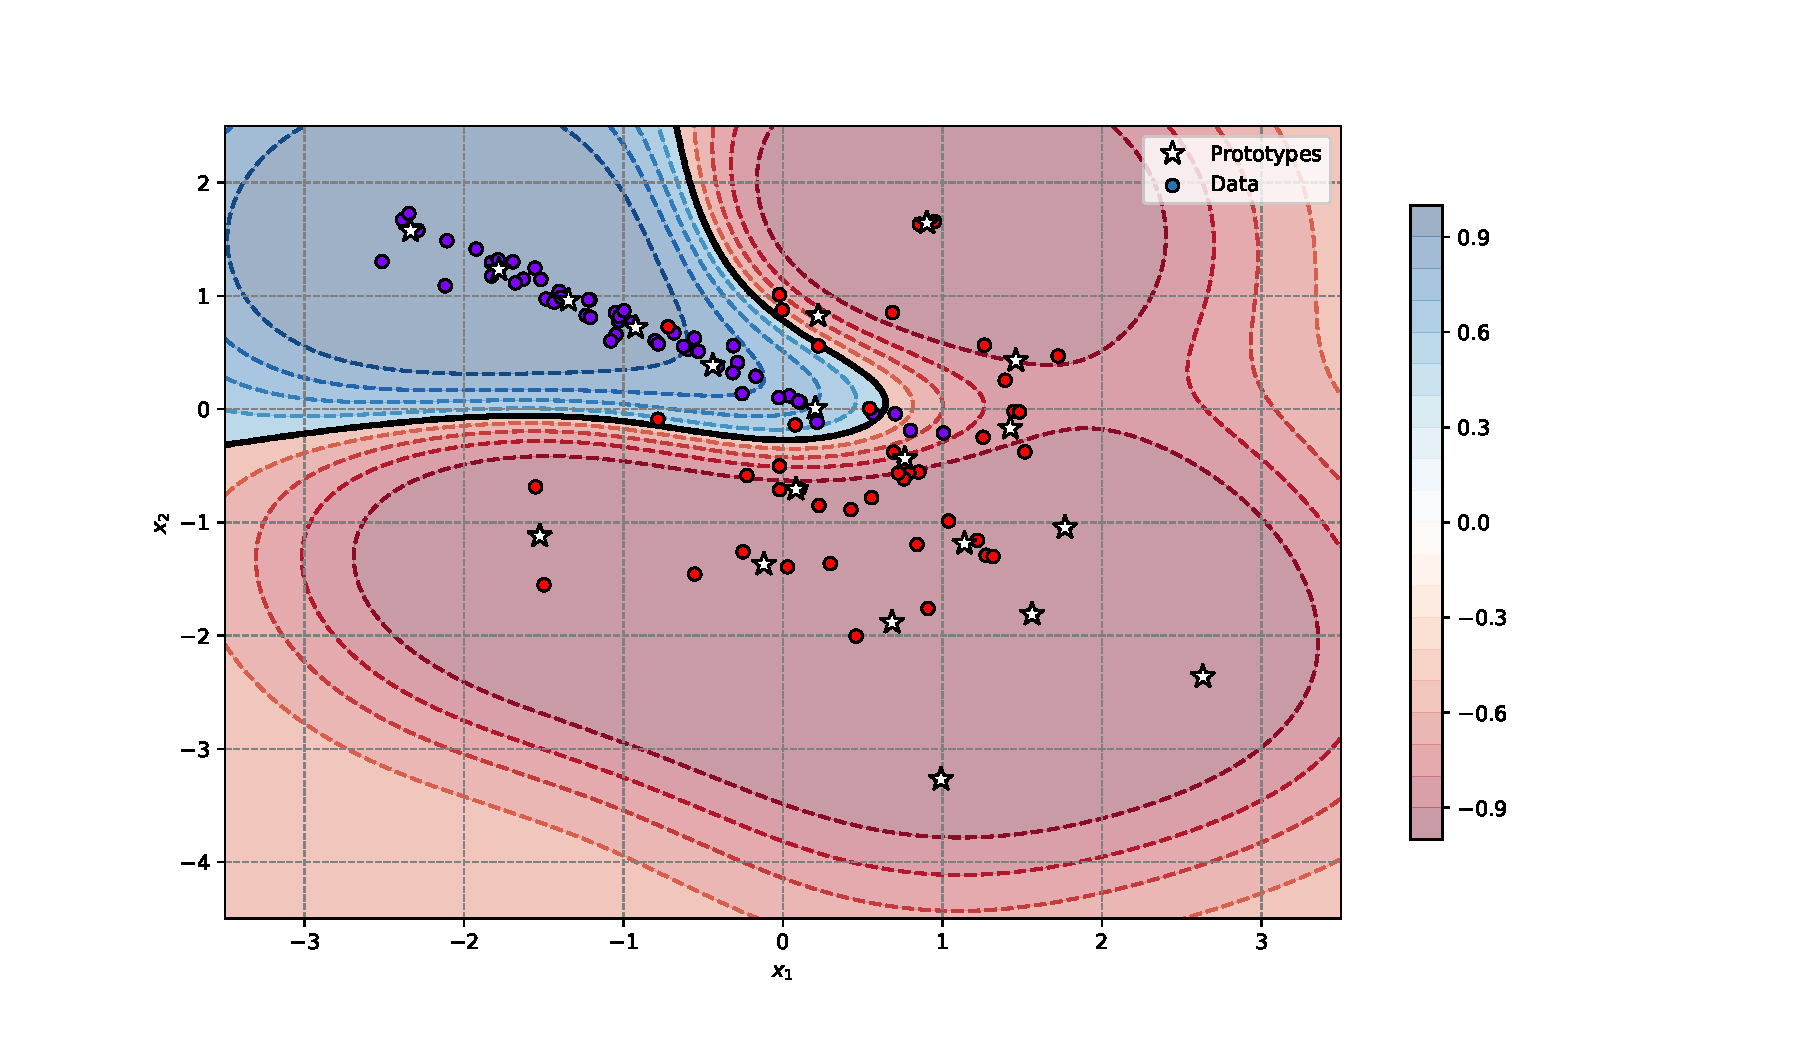
\includegraphics[scale=0.55]{10_deep_learning/02_img/rbfn}
	\end{figure}
\end{frame}


% Section: Multi-Layer-Perceptrons (MLPs)
%______________________________________________________________________
\section{Multi-Layer-Perceptrons (MLPs)}
\makedivider{Multi-Layer-Perceptrons (MLPs)}

% Subsection: Backpropagation
% --------------------------------------------------------------------------------------------------------
\subsection{Backpropagation}

% Backpropagation
\begin{frame}{Backpropagation}{}
	\begin{itemize}
		\item To calculate the error, we first have to perform a forward pass:
		\begin{equation*}
			h_k(\bm{x}^{(i)}) = g^{(2)}\left( \sum_{l=0}^h \Theta_{kl}^{(2)} g^{(1)}\left( \sum_{j=0}^d \Theta_{lj}^{(1)} x_{j}^{(i)} \right) \right)
		\end{equation*}
		\item The loss function is given by:
		\begin{equation*}
			\mathcal{J}^{(i)}(\bm{\Theta}) = \frac{1}{n} \sum_{i=1}^n \sum_{k=1}^{\vert \mathcal{C} \vert}
				\ell(h_k(\bm{x}^{(i)}; \bm{\Theta}), y_k^{(i)})
		\end{equation*}
	\end{itemize}
\end{frame}


% Backpropagation (Ctd.)
\begin{frame}{Backpropagation (Ctd.)}{}
	\begin{itemize}
		\item Compute the gradient w.\,r.\,t. $h_k$:
		\begin{equation*}
			\nabla_{h_k} \mathcal{J}^{(i)}(\bm{\Theta}) = \ell'(h_k(\bm{x}^{(i)}; \bm{\Theta}), y_k^{(i)}) \equiv \delta_k^{(i)}
		\end{equation*}
		\item Now we can compute the weight gradients:
		\footnotesize
		\begin{align*}
			\nabla_{\Theta_{kl}^{(2)}} \mathcal{J}^{(i)}(\bm{\Theta})
				&= \frac{\partial \mathcal{J}^{(i)}(\bm{\Theta})}{\partial h_k(\bm{x}^{(i)}; \bm{\Theta})}
					\frac{\partial h_k(\bm{x}^{(i)}; \bm{\Theta})}{\partial \Theta_{kl}^{(2)}} \\
				&= \ell'(h_k(\bm{x}^{(i)}; \bm{\Theta}), y_k^{(i)}) \cdot g'^{(2)} \left( \sum_{t=0}^h \Theta_{kt}^{(2)} z_t(\bm{x}^{(i)}) \right)
					\cdot z_l(\bm{x}^{(i)}) \\
				&= \delta_k^{(i)} \cdot g'^{(2)} \left( \sum_{t=0}^h \Theta_{kt}^{(2)} z_t(\bm{x}^{(i)}) \right) \cdot z_l(\bm{x}^{(i)})
		\end{align*}
	\end{itemize}
\end{frame}



% Section: Wrap-Up
%______________________________________________________________________
\section{Wrap-Up}
\makedivider{Wrap-Up}

% Subsection: Summary
% --------------------------------------------------------------------------------------------------------
\subsection{Summary}

% Summary
\begin{frame}{Summary}{}
	\begin{itemize}
		\item 
	\end{itemize}
\end{frame}


% Subsection: Self-Test Questions
% --------------------------------------------------------------------------------------------------------
\subsection{Self-Test Questions}

% Self-Test Questions
\begin{frame}{Self-Test Questions}{}\important
	\begin{enumerate}
		\item
	\end{enumerate}
\end{frame}


% Subsection: Lecture Outlook
% --------------------------------------------------------------------------------------------------------
\subsection{Lecture Outlook}

\begin{frame}{What's next...?}{}
	\makeoverview{8}
\end{frame}


% Subsection: Recommended Literature and further Reading
% --------------------------------------------------------------------------------------------------------
\subsection{Recommended Literature and further Reading}

% Literature
%______________________________________________________________________
\begin{frame}{Recommended Literature and further Reading}{}
	\footnotesize
	\begin{thebibliography}{2}
		\literature{book}{Goodfellow.2016}{[2] Deep Learning}
			{Ian Goodfellow et al. MIT Press. 2016.}{$\rightarrow$ \href{
				http://www.deeplearningbook.org/
			}{\linkstyle{Link}}, cf. chapters 6 \textit{Deep Feedforward Networks}, especially chapter 6.5}
	
		\literature{book}{Bishop.2006}{[2] Pattern Recognition and Machine Learning}
			{Christopher Bishop. Springer. 2006.}{$\rightarrow$ \href{
				http://users.isr.ist.utl.pt/~wurmd/Livros/school/Bishop\%20-\%20Pattern\%20Recognition\%20And\%20Machine\%20Learning\%20-\%20Springer\%20\%202006.pdf
			}{\linkstyle{Link}}, cf. chapter 5 \textit{Neural Networks}, especially chapter 5.3}

	\end{thebibliography}
\end{frame}


% Thank you
%______________________________________________________________________
\makethanks

\end{document}